
%!TEX ROOT=main.tex


\part{Realization}
\label{chap:realization}
Since there are no spare parts available for the transmitter or the car, all modifications have been made with as little structural intervention as possible. This process can be referred to as retrofitting.

\section{Transmitter}
\label{sec:real_tx}
\subsection{Power supply}
As described in section \ref{sec:hw_mods}, the transmitter is powered by a 2-cell LiPo battery with a nominal voltage of \SI{7.4}{\V}. The battery is connected via an XT60 connector and a switch to a step-down converter module with an LM2596 chip. The module is needed to regulate the battery voltage to \SI{5}{\V} to power the control board.

This voltage is used for the RGB LED, communication module, and linear voltage regulator AP2111, which regulates it to \SI{3.3}{\V} used to power the rest of the components. This regulator was selected because of the low dropout voltage of only \SI{250}{\mV} and high output current of \SI{600}{\mA} \cite{ap_datasheet}.		%TODO measure TX current?

In order to measure the battery voltage with the processor's internal ADC, it first had to be lowered to fit within the ADC range, which is $0\, \text{-}\, 3.3$\unit{\V}. Therefore a voltage divider is soldered to the input terminals of the step-down module. The divider was designed to use resistors with standard values and is pictured in figure \ref{fig:tx_div}. The resistor values are R1 = \SI{22}{\kohm}, R2 = \SI{10}{\kohm}.
\begin{figure}[ht]
\centering
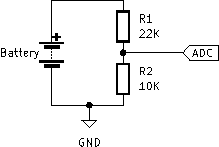
\includegraphics[width=0.4\linewidth]{fig/voltage_divider.pdf}
\caption{Voltage divider utilized in the transmitter }
\label{fig:tx_div}
\end{figure}

A fully charged 2-cell LiPo battery reaches \SI{8.4}{\V}, then the output of the divider equals
\begin{equation}
	U_{adc} = U_{batt} \cdot \frac{R2}{R1+R2} = \SI{2.625}{\V}\ ,
\end{equation}
which is safely within the ADC range.

\subsection{Controls}
The transmitter was supplied with a steering wheel and trigger as 5kohm potentiometers. Since they are old, a \SI{100}{\nF} capacitor was added between the output pin of both potentiometers and ground to form a low-pass filter and smooth out the output signal.

Potentiometers used for control trimming were replaced with quadrature rotary encoders with push buttons. Encoders have screw threads, as can be seen in figure *fig*, which fit into the original holes. Since encoders are fixed to the transmitter, a simple connector made from a pin socket was soldered to encoder pins [TODO: fotka].

\subsection{PCB design}